% !TeX spellcheck = en_US
%%
%% sample document for AAMAS'18 conference
%%
%% modified from sample-sigconf.tex
%%
%% see ACM instructions acmguide.pdf
%%
%% AAMAS-specific questions? n.yorke-smith@tudelft.nl
%%

\documentclass[sigconf]{aamas}  % do not change this line!

%% your usepackages here, for example:
\usepackage{booktabs}
\usepackage{graphicx}
\usepackage[rflt]{floatflt}
\usepackage{subcaption} 
\usepackage{frame, caption}
\usepackage{amsmath}
\usepackage{mathrsfs}
\usepackage{array}

\newcommand{\argmax}{\operatornamewithlimits{arg\,max}}

%% do not change the following lines
\setcopyright{ifaamas}  % do not change this line!
\acmDOI{doi}  % do not change this line!
\acmISBN{}  % do not change this line!
\acmConference[AAMAS'18]{Proc.\@ of the 17th International Conference on Autonomous Agents and Multiagent Systems (AAMAS 2018), M.~Dastani, G.~Sukthankar, E.~Andre, S.~Koenig (eds.)}{July 2018}{Stockholm, Sweden}  % do not change this line!
\acmYear{2018}  % do not change this line!
\copyrightyear{2018}  % do not change this line!
\acmPrice{}  % do not change this line!

%% the rest of your preamble here


%%%%%%%%%%%%%%%%%%%%%%%%%%%%%%%%%%%%%%%%%%%%%%%%%%%%%%%%%%%%%%%%%%%%%%%%%%%%%%%%%%%%%%%%%%%%%%%%%%%%%%%%%

%%%%%%%%%%%%%%%%%%%%%%%%%%%%%%%%%%%%%%%%%%%%%%%%%%%%%%%%%%%%%%%%%%%%%%%%%%%%%%%%%%%%%%%%%%%%%%%%%%%%%%%%%

\begin{document}
	
	\title{I've got the power's value! A computational model to evaluate the interlocutor's behaviors in collaborative negotiation}  % put your title here!
	%\titlenote{Produces the permission block, and copyright information}
	
	% AAMAS: as appropriate, uncomment one subtitle line; check the CFP
	%\subtitle{Extended Abstract}
	%\subtitle{Industrial Applications Track}
	\subtitle{Socially Interactive Agents Track}
	%\subtitle{Blue Sky Ideas Track}
	%\subtitle{Robotics Track}
	%\subtitle{JAAMAS Track}
	%\subtitle{Doctoral Mentoring Program}
	
	%\subtitlenote{The full version of the author's guide is available as \texttt{acmart.pdf} document}
	
	
	% AAMAS: submissions are anonymous for most tracks
	\author{Paper \#32}  % put your paper number here!
	
	%% example of author block for camera ready version of accepted papers: don't use for anonymous submissions
	%
	%\author{Ben Trovato}
	%\authornote{Dr.~Trovato insisted his name be first.}
	%\orcid{1234-5678-9012}
	%\affiliation{%
	%  \institution{Institute for Clarity in Documentation}
	%  \streetaddress{P.O. Box 1212}
	%  \city{Dublin} 
	%  \state{Ohio} 
	%  \postcode{43017-6221}
	%}
	%\email{trovato@corporation.com}
	%
	%\author{G.K.M. Tobin}
	%\authornote{The secretary disavows any knowledge of this author's actions.}
	%\affiliation{%
	%  \institution{Institute for Clarity in Documentation}
	%  \streetaddress{P.O. Box 1212}
	%  \city{Dublin} 
	%  \state{Ohio} 
	%  \postcode{43017-6221}
	%}
	%\email{webmaster@marysville-ohio.com}
	%
	%\author{Lars Th{\o}rv{\"a}ld}
	%\authornote{This author is the
	%  one who did all the really hard work.}
	%\affiliation{%
	%  \institution{The Th{\o}rv{\"a}ld Group}
	%  \streetaddress{1 Th{\o}rv{\"a}ld Circle}
	%  \city{Hekla} 
	%  \country{Iceland}}
	%\email{larst@affiliation.org}
	%
	%\author{Valerie B\'eranger}
	%\affiliation{%
	%  \institution{Inria Paris-Rocquencourt}
	%  \city{Rocquencourt}
	%  \country{France}
	%}
	%\author{Aparna Patel} 
	%\affiliation{%
	% \institution{Rajiv Gandhi University}
	% \streetaddress{Rono-Hills}
	% \city{Doimukh} 
	% \state{Arunachal Pradesh}
	% \country{India}}
	%\author{Huifen Chan}
	%\affiliation{%
	%  \institution{Tsinghua University}
	%  \streetaddress{30 Shuangqing Rd}
	%  \city{Haidian Qu} 
	%  \state{Beijing Shi}
	%  \country{China}
	%}
	%
	%\author{Charles Palmer}
	%\affiliation{%
	%  \institution{Palmer Research Laboratories}
	%  \streetaddress{8600 Datapoint Drive}
	%  \city{San Antonio}
	%  \state{Texas} 
	%  \postcode{78229}}
	%\email{cpalmer@prl.com}
	%
	%\author{John Smith}
	%\affiliation{\institution{The Th{\o}rv{\"a}ld Group}}
	%\email{jsmith@affiliation.org}
	%
	%\author{Julius P.~Kumquat}
	%\affiliation{\institution{The Kumquat Consortium}}
	%\email{jpkumquat@consortium.net}
	%
	%% The example's default list of authors is too long for headers
	%\renewcommand{\shortauthors}{B. Trovato et al.}
	
	
	\begin{abstract}  % put your abstract here!
		
		Interpersonal dominance relation has a major effect on the outcome of a negotiation. It has been shown that when participants adopt complementary dominance behaviors (one being dominant and the other being submissive), they reach mutually beneficial outcomes and this increases their reciprocal likings. In this paper, we investigate about the simulation of this interpersonal relationship in the context of collaborative negotiation between artificial agents.
		
		Our simulation is based on a previously published model. We present a Theory of Mind model that allows an agent to evaluate its interlocutor's level of dominance. The agent establishes the relation of dominance by adapting its behavior of power to complement the power of its interlocutor. We show on agent-agent simulation that the system correctly predicts the interlocutor's power. 
		
	\end{abstract}
	
	
	% AAMAS: the ACM CCS are not needed within AAMAS papers
	%%
	%% The code below should be generated by the tool at
	%% http://dl.acm.org/ccs.cfm
	%% Please copy and paste the code instead of the example below. 
	%%
	%\begin{CCSXML}
	%<ccs2012>
	% <concept>
	%  <concept_id>10010520.10010553.10010562</concept_id>
	%  <concept_desc>Computer systems organization~Embedded systems</concept_desc>
	%  <concept_significance>500</concept_significance>
	% </concept>
	% <concept>
	%  <concept_id>10010520.10010575.10010755</concept_id>
	%  <concept_desc>Computer systems organization~Redundancy</concept_desc>
	%  <concept_significance>300</concept_significance>
	% </concept>
	% <concept>
	%  <concept_id>10010520.10010553.10010554</concept_id>
	%  <concept_desc>Computer systems organization~Robotics</concept_desc>
	%  <concept_significance>100</concept_significance>
	% </concept>
	% <concept>
	%  <concept_id>10003033.10003083.10003095</concept_id>
	%  <concept_desc>Networks~Network reliability</concept_desc>
	%  <concept_significance>100</concept_significance>
	% </concept>
	%</ccs2012>  
	%\end{CCSXML}
	%
	%\ccsdesc[500]{Computer systems organization~Embedded systems}
	%\ccsdesc[300]{Computer systems organization~Redundancy}
	%\ccsdesc{Computer systems organization~Robotics}
	%\ccsdesc[100]{Networks~Network reliability}
	
	
	\keywords{Dominance; Reasoning about other; Theory of mind}  % put your semicolon-separated keywords here!
	
	\maketitle
	
	
	%%%%%%%%%%%%%%%%%%%%%%%%%%%%%%%%%%%%%%%%%%%%%%%%%%%%%%%%%%%%%%%%%%%%%%%%%%%%%%%%%%%%%%%%%%%%%%%%%%%%%%%%%
	%% start of main body of paper
	%
	
	\section{Introduction}
	Negotiation is a common task in daily life. People negotiate not only in professional situations (\emph{e.g.} for a salary increase or a promotion) but also in more simple situations such as choosing the movie to watch or the holiday destination. In the last decade, a variety of conversational agents have been created to negotiate with people \cite{pynadath2013you,gratch2016misrepresentation,klatt2011negotiations}. Theses agents are designed with a growing number of decisional abilities, including multi-party and multi-issues negotiation capabilities.
	
	However, negotiation is a multifaceted process which also involves social interaction and affects as well as personal preferences and opinions  \cite{bro2010affective}. Several research considered the role social behavior in the negotiation process. For instance, [ref-marsella] studied the impact of emotion on the outcome of the negotiation. [ref-elisabetta] studied how the expression of social attitudes at the non-verbal level changes the perception of the negotiation.
	
	One key element in the social aspect of negotiation is the interpersonal relation between the participants. Indeed, researches in social psychology demonstrated that the relation of dominance affects the way the negotiation process is perceived \cite{van2006power}. Negotiating parties often differ in terms of dominance and this difference exerts an important influence on the behavior of participants. Negotiators build different negotiation strategies depending on their relative dominance. This directly influences the outcomes of the negotiation. More precisely, Tidens \cite{tiedens2003power} showed that dominance complementarity (\emph{i.e.} one negotiator exhibits dominant behaviors while the other one responds with submissive ones) leads the negotiators to reach mutually beneficial outcomes and increases their reciprocal likings. \cite{wiltermuth2015benefits,tiedens2003power}.
	
	For this reason, it is important to develop negotiator agents that can adapt their social behavior to the dominance of their interlocutor. Our work aims at developing such a system that is capable of evaluating and adapting to this degree of dominance.
	
	We focus on a specific kind of interaction called \emph{collaborative negotiation}. Unlike adversarial negotiation, collaborative negotiation assumes that each participant is driven by the goal of finding a trade-off that best satisfies the interests of all the participants as a group, instead of one that maximizes his own interest\cite{sidner1994artificial,chu1995response}. In order to develop our adaptative negotiator agent, we first designed a model of collaborative negotiation that allows an agent to express its social dominance through negotiation strategies \cite{ouali2017computational}. We showed that human observers correctly perceive the dominance expressed by the agent. The next steps are to evaluate the level of dominance of the interlocutor and to adapt the agent's level of dominance. In this paper, we present a theory of mind approach to evaluate the level of dominance of the interlocutor (step 2 on Figure~\ref{fig:schema-general}).

	\begin{figure*}
			\fbox{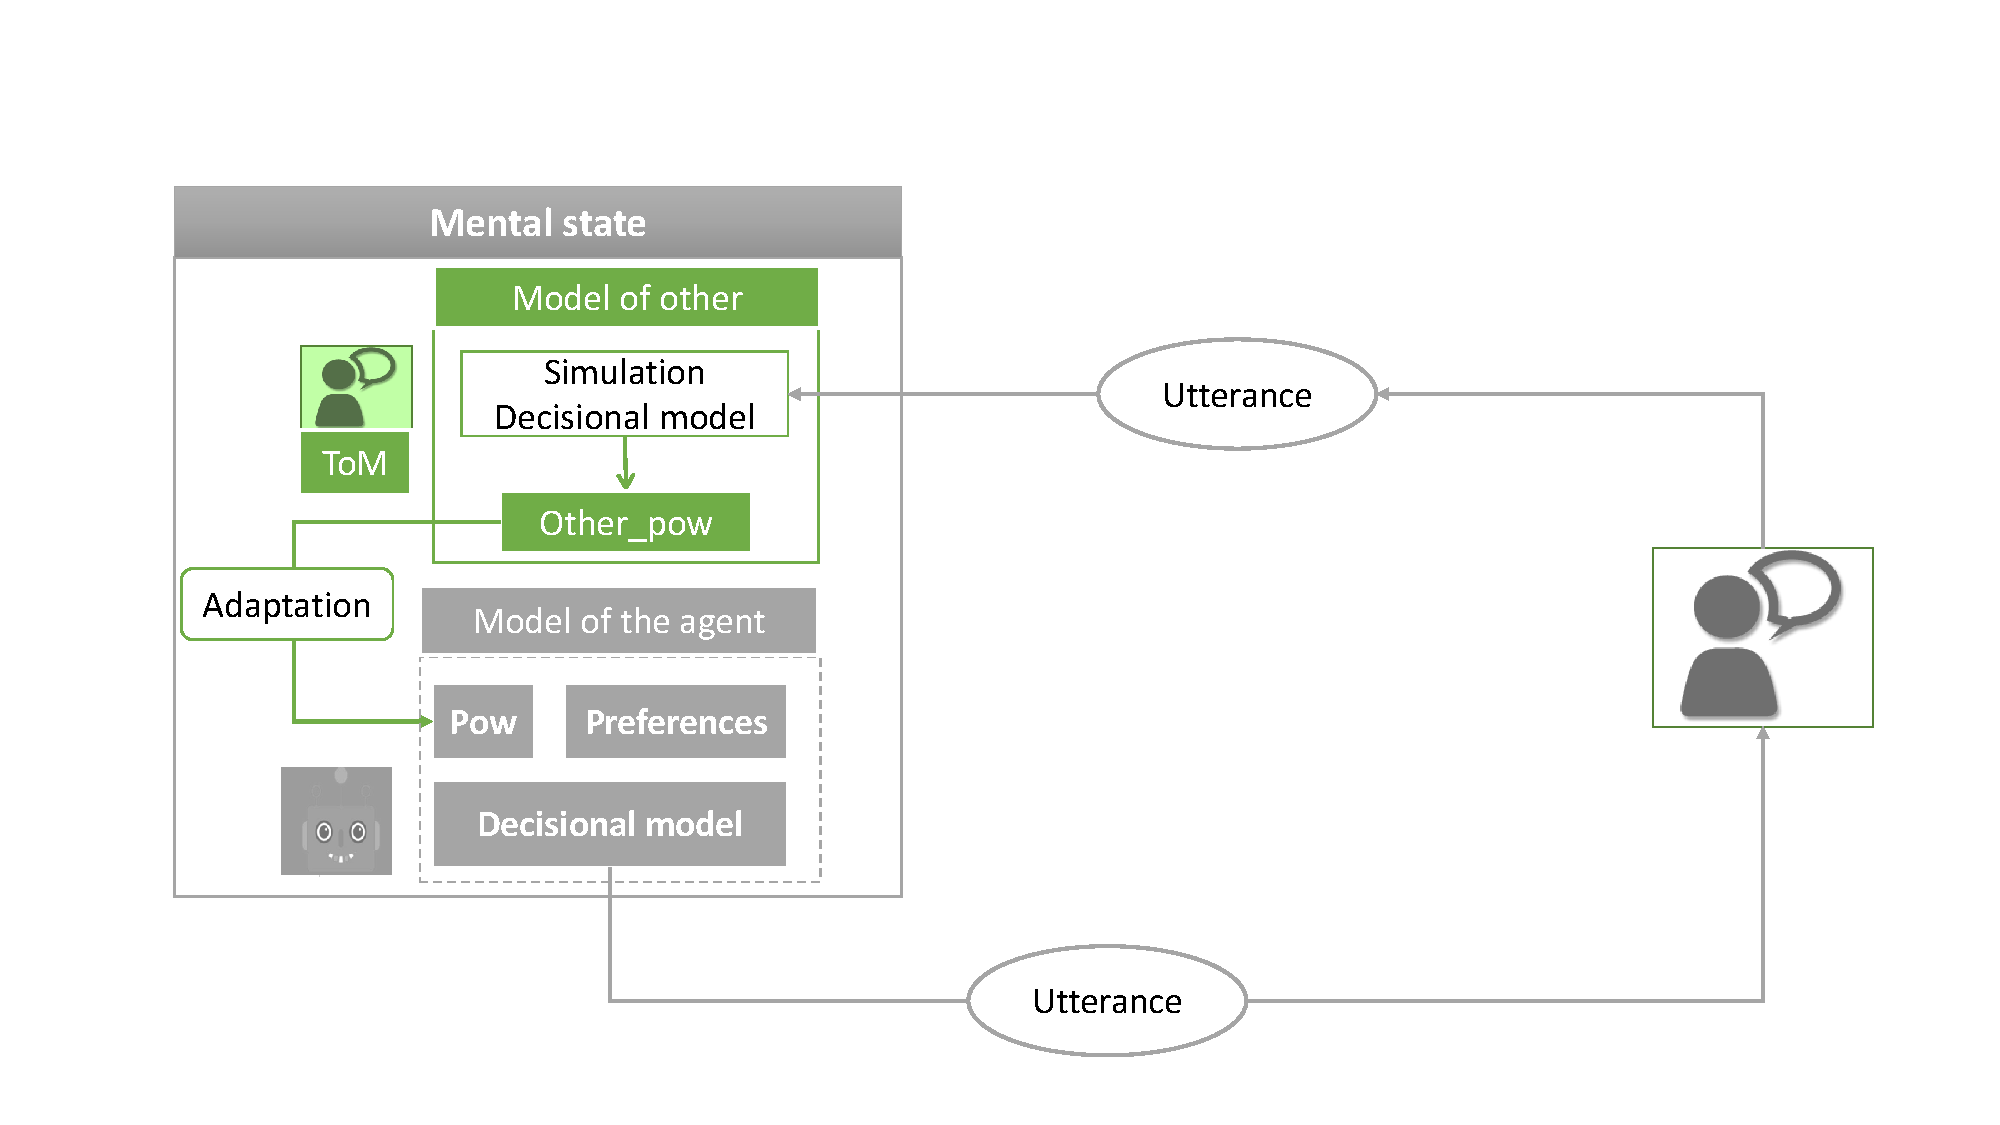
\includegraphics[width=\linewidth, height= 0.4\textheight]{figs/model_tom.pdf}}
			\caption{Model of collaborative negotiation with a model of other} 
			\label{fig:schema-general}
	\end{figure*} 
	
%	
%	
%	 that allows the agent to establish a complementary relation of dominance with the user. Thus, the agent adapts its behaviors to complement the behaviors of the user. 
%	
%	To construct a complementary relation of dominance, the agent has to predict the user's behaviors of power in order to adapt a complementary strategy. 
%	%il manque qlq chose
%	In a previous work \cite{ouali2017computationall}, we designed a negotiation agent capable of expressing negotiation's strategies that reflect his level of power. We propose to extend this model, with theory of mind abilities based on simulation, that allow the agent to simulate the decisional model of tis partner and predict his level of dominance.
%	
%	Since the implemented behaviors of power reflect human behaviors, we assume that the user uses the same decision model to negotiate. Therefore, the agent will define beliefs about the user's reasoning model based on the utterances expressed. 
%	
%	
%	In this paper specifically, we present our model of theory of mind that constructs a mental model of the user and processes the value of power he exhibits in the negotiation. 
%	
	The paper is organized as follows. Section II gives an overview of previous automated negotiation agents with theory of mind and other related work on social behavior recognition. In section III, we briefly present our model of dialogue for collaborative negotiation. We show that extendeding this model with a theory of mind raises computational issues. We propose a new model to evaluate the dominance of the interlocutor. This model is based on reasoning with uncertainty. Section IV presents an evaluation of this new model in the context of agent-agent negotiation. We show that the system correctly predicts the interlocutor's power in spite of the restrictions on the model. In section V, we discuss the future use of this new model for building an adaptative negotiator agent.
	
	
	\section{Related works}
	
	In social interactions and negotiation in particular, reasoning about the beliefs, goals, and intentions of others is crucial. People use this so-called theory of mind \cite{premack1978does} or mentalizing to understand why others behave the way they do, as well as to predict the future behavior of others. Therefore, various negotiation models use theory of mind approaches to create  more realistic models of negotiation. 
	
	For instance, Pynadath \textit{et al}\cite{pynadath2013you} showed the advantages of theory of mind on negotiation even with an overly simplified model. They observed significant similarities between	the partner behaviors and the agent's idealized expectations. Moreover, deviations in expectations about the other did not affect the agent performances and played in some cases in the advantage of the agent.
	
	De Weerd \textit{et al} \cite{de2013higher} also investigated the use of high-order theory of mind in mixed-motive situations where cooperative and competitive behaviors play an important role. They found that the use of first-order and second-order theory of mind allow agents to balance competitive and cooperative	aspects of the game. This prevents agents from breaking down compared to  agents without theory of mind.
	
	
	Both approaches only focus on rational behaviors and exclude social aspects. However, the impact of social behaviors has been extensively debated in social psychology. Among such works, various researches have been investigating emotion recognition in negotiation; the effects of one individual's	emotions on the other's social decisions and behavior during the negotiation. Moreover, they investigate how theses resource of information are integrated.
	For example, Elfenbein\textit{ et al} \cite{elfenbein2007reading} proved that  emotion recognition accuracy is positively correlated to  better performances in negotiation
	
	In the same vein, several researches suggested that anger expression has effects on the negotiation \cite{sinaceur2006get,van2010interpersonal,ferguson2004social}. For example, VanKleef \cite{van2004interpersonal} demonstrated that negotiators monitor their opponent's emotions and use them to estimate the opponent's limits, and modify their demands according to the presumed location of those limits. As a result, negotiators concede more to an angry opponent than to a happy one. 
	
	
	For theses reasons, reasoning about the social behaviors is important for the percpective of constructing negotiators agents. \cite{alfonso2015emotional} proposed a model that can observe and predict other's agents emotional behaviors. The three step method proposes to revise the agent's  beliefs by integrating a Bayesian model which infers probabilities about the emotional behaviors of other's agents and compute probabilistic prediction about their appraisals.
	
	Marcella \textit{et al} \cite{klatt2011negotiations} proposed a model of negotiation in the context of aid prevention. The model tries to combine handling of emotions with general structures of negotiations. 
	
	In the context our work, we focus on the impact of dominance in the negotiation. Dominance as an interpersonal relation is defined by burgoon \cite{burgoon1998nature} as expressive, relationally based communicative acts by which power is exerted and influence achieved. Furthermore, it is a dyadic variable in which control attempts by one individual are accepted by the
	interactional partner \cite{dunbar2005perceptions}. For this reason, we focus on dominance complementarity between a negotiator agent and a human user in the context of collaborative negotiation. 
	
	Dominance complementarity is characterized by one person in a dyadic interaction behaving dominantly and his counterpart behaving submissively \cite{tiedens2003power} and those behaviors have been investigated in the context of negotiation. \cite{tiedens2003power} showed that when complementarity occurs in an interaction, people feel more comfortable and helps to create interpersonal liking relation.
	Moreover, \cite{wiltermuth2015benefits} showed that dominance complementarity can positively improve coordination and by consequences improve objective benefits.
	
	Our goal is to create a model of negotiation in which the agent adapts its negotiation strategies to the relation of dominance established with the user. Therefore, the agent has to reason about user's behaviors of \emph{power} to understand the level of dominance or submissiveness expressed. The agent then adopt a complementary strategy in order to complement the user behaviors and establish the relation of dominance.
	
	We present in this paper a model of theory of mind that builds beliefs about the user behaviors of power in order to predict his behavior of dominance. We propose to use our model of negotiation based on power in order to reason about the user behaviors. 


\section{Model of collaborative negotiation}
	
	Our simulation of interpersonal relation of dominance is based on a previously proposed model of collaborative negotiation \cite{x}. In this model, the artificial agent selects an utterance based on the previously exchanged information and on its personal level of social power, represented as a variable in [0,1]. We showed that the dialogues produced by this model allow human users to correctly perceive the different dimensions of social power expressed by the agent.
	
	Our goal is to use this dialogue model to simulate the interlocutor's behavior. From a given utterance produced by the interlocutor, the agent will try to evaluate the level of power by comparing this utterance with the possible outcomes of the dialogue model.
	
	It is not necessary to have a complete knowledge of this dialogue model to understand the simulation presented here. However, some elements are required to explain our approach. This section briefly presents the main principles of the collaborative negotiation dialogue model.
	
	\subsection{Dialogue model}
	\label{sec:dialogue-model}
	
%	We defined a dialogue system of collaborative negotiation which enable  a conversational agent to create and adapt its negotiation strategy to the power it intends to express. 
	The goal of a negotiation is to choose an option in a set of possible values $\mathcal{O}$. Each option $o\in\mathcal{O}$ is defined as a set of values $\{v_1, ..., v_n\}$ associated to criteria $\{C_1, ..., C_n\}$ that reflect the options characteristics.  For instance, in a negotiation about restaurants, the criteria might be the type of cuisine and the price, we could have the option: $(French,expensive)$.
	
	The agent is provided with a set of partial or total ordered preferences $\prec_i$ defined for each criterion $C_i$. For example, the agent prefers Chinese food to Turkish one. Using theses preferences, it can compute a score of satisfaction $sat(v)$ for each value of each criterion. The satisfaction of a value $v \in C_i$ is computed as the number of values that the agent prefers less in the preferences order $\prec_i$.
	%, then, the score is normalized in $[0, 1]$: 
	
%	\begin{equation}
%	sat(v, \prec_i) =	1 - \left( \frac{|\{v' : v' \neq v \  \wedge \ (v \prec_i v')\}| }{( |C_i| - 1 )}\right)
%	\end{equation}
%	
	The notion of satisfaction represents the score of liking for the value. The closer the satisfaction of a value $v$ gets to 1, the more the agent likes $v$.
	
	\par For example, let us consider a domain $M =\{A, B, C, D\}$ with the set of preferences $\{A \prec B, C \prec D , B \prec D \}$. The values of satisfiability are depicted in the table \ref{tab:sat}.
		\begin{table}
			\centering
			\begin{tabular}{ |c|c|c|c|c| }
				\hline				
				value & A & B & C & D \\
				\hline
				
				\hline
				sat(value) & 0.3 & 0.6 & 0.6 & 1 \\
				\hline
				
			\end{tabular}
			\caption{Value of satisfiability for the model $M$.}
			\label{tab:sat}
		\end{table}
	
	\par
	In our model, agents communicate using 5 utterances types: \emph{AskPreference} and \emph{StatePreference} to exchange information about the preferences; \emph{Propose}, \emph{Accept} and \emph{Reject} to make negotiation moves. The selection of these utterance types and the values is based on the decision model related to power presented hereafter.
	
	\subsection{Decision based on power}
	
	The decisional process is built to take into account the power of the agent, its preferences and the context of the negotiation. Therefore, the agent is initiated with a value of power $pow \in [0,1]$. 
	
	The selection of the utterance relies on three elements.
	
	\subsubsection{Lead of the dialogue}
	De Dreu showed that the participant with higher power tends to lead the dialogue and to focuses on the negotiation convergence \cite{magee2007power,de2004influence}. In our model, this means that agents with high values of power ($pow>0.5$) will select \emph{Propose} moves more often. On the contrary, submissive negotiators focus on having accurate knowledge about the other to take the fairest decision. In our model, agents with low power will select \emph{AskPreferences} utterances more often to collect information.
		
	\subsubsection{Satisfiability: StatePreferences}
	\label{sec:sat}
	When using a \emph{StatePreference(v)} utterance, the agent expresses its liking for a value. As showed by \cite{de1995impact}, high-power negotiators are more demanding than low-power ones. For this reason, in our model, the set of values that the agent likes, named $S$, depends on the level of power $pow$. It is computed as follows:
	\begin{equation}
	\forall v,\hspace{2mm} v\in S\hspace{2mm}\mathrm{iff}\hspace{2mm}sat(v) \geq pow
	\end{equation}
	
	For example, if we consider the preference set given on table~\ref{tab:sat} and the power $pow=0.6$, we can compute the set of satisfiable values $S = \{B, C, D\}$. This set $S$ is used directly to compute the values of \emph{StatePreference} utterances.
	
	\subsubsection{Acceptability: negotiation moves}
	During the negotiation, the agent makes decisions about the proposals it receives. It might express an \emph{Accept} or \emph{Reject}. However, in the context of collaborative negotiation, participants make concessions when the discussion is not converging. In our dialogue model, this means that the agent has to lower his level of demand.
	
		\begin{floatingfigure}[r]{1.5in}
			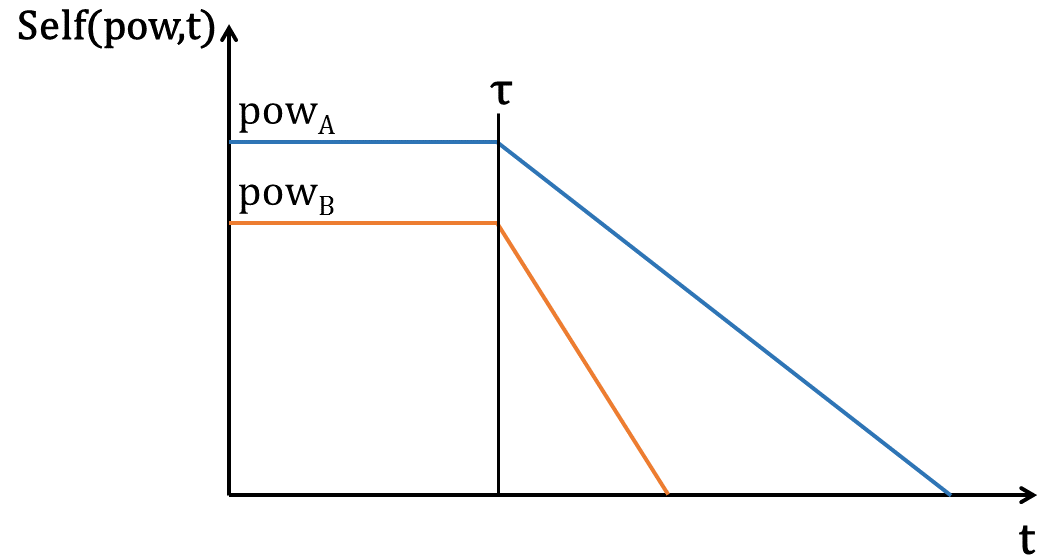
\includegraphics[width=1.5in]{figs/sv3.png}
			\caption{\label{fig:conc}Concession curve}
		\end{floatingfigure} 
		
	For this reason, we define the variable $self(t)$ which is a time varying function of $pow$, decreasing over time $t$. In the beginning, $self(0) = pow$ and when the negotiation evolves without converging, self decreases as presented in the figure \ref{fig:conc}. The concession slope is stronger for low-power agents.
	
	This value of $self$ is used directly to answer a \emph{Propose(v)} utterance. We say that the value $v$ is \emph{acceptable} at time $t$, and we note $v \in Ac$, when:
	\begin{equation}
	v\in Ac\hspace{2mm}\mathrm{iff}\hspace{2mm}sat(v) \geq self(t)
	\end{equation}
	
	The agent will answer with an \emph{Accept} to a proposal only if the value is acceptable, and will answer with a \emph{Reject} otherwise. Also note that, when building proposals (i.e. \emph{Propose} utterances) the agent can only propose a value that is acceptable.
	
	Finally, it is important to note that the set $Ac$ grows over time: as the negotiation evolves, the agent might accept proposals which are not satisfiable, as a consequence of making concessions. We denote $M\varsubsetneq Ac$ the set of not-satisfiable values that can be accepted in the current dialogue move: $M = Ac\setminus S$.
	
	\subsubsection{Summary}	
	Table~\ref{tab:utt} presents the applicability condition for the five utterance types, based on the values of $pow$ and the derived sets $S$ and $Ac$. The utterance \emph{AskPreference} only depends on the lead of dialogue rules, related to the value of $pow$.
		
		\begin{table}
			\centering
				\caption{Applicability conditions for the five utterance types.}
				\label{tab:utt}
			\begin{tabular}  {|l|l|}
				\hline
				Utterance & Applicability condition \\
				\hline
				AskPreference(v) & None \\
				\hline 
				StatePreference(v) & $v\in S$ \\
				\hline 
				Propose(v) & $v\in Ac$ \\
				\hline
				Accept(v)  & $v\in Ac$ \\
				\hline
				Reject(v) & $v\notin Ac$ \\
				\hline
			\end{tabular}
		\end{table}
	
	\subsection{Beliefs about other: general algorithm}
	
	In order to build a complementary relation of dominance with the user, the agent has to evaluate the power of the user, as presented in figure \ref{fig:schema-general}. To this goal, we propose to use a Theory of Mind (ToM) approach \cite{premack1978does}. The idea is to consider different hypotheses about the user's mental state, including his/her value of power. Using the decision model, we simulate the possible proposals, questions or answers that can be produced. We then compare the result of this simulation with the actual utterance expressed by the user. This gives information about the possible values of power. This idea is illustrated on Figure~\ref{fig:tom}.
		
	\begin{figure*}
			\fbox{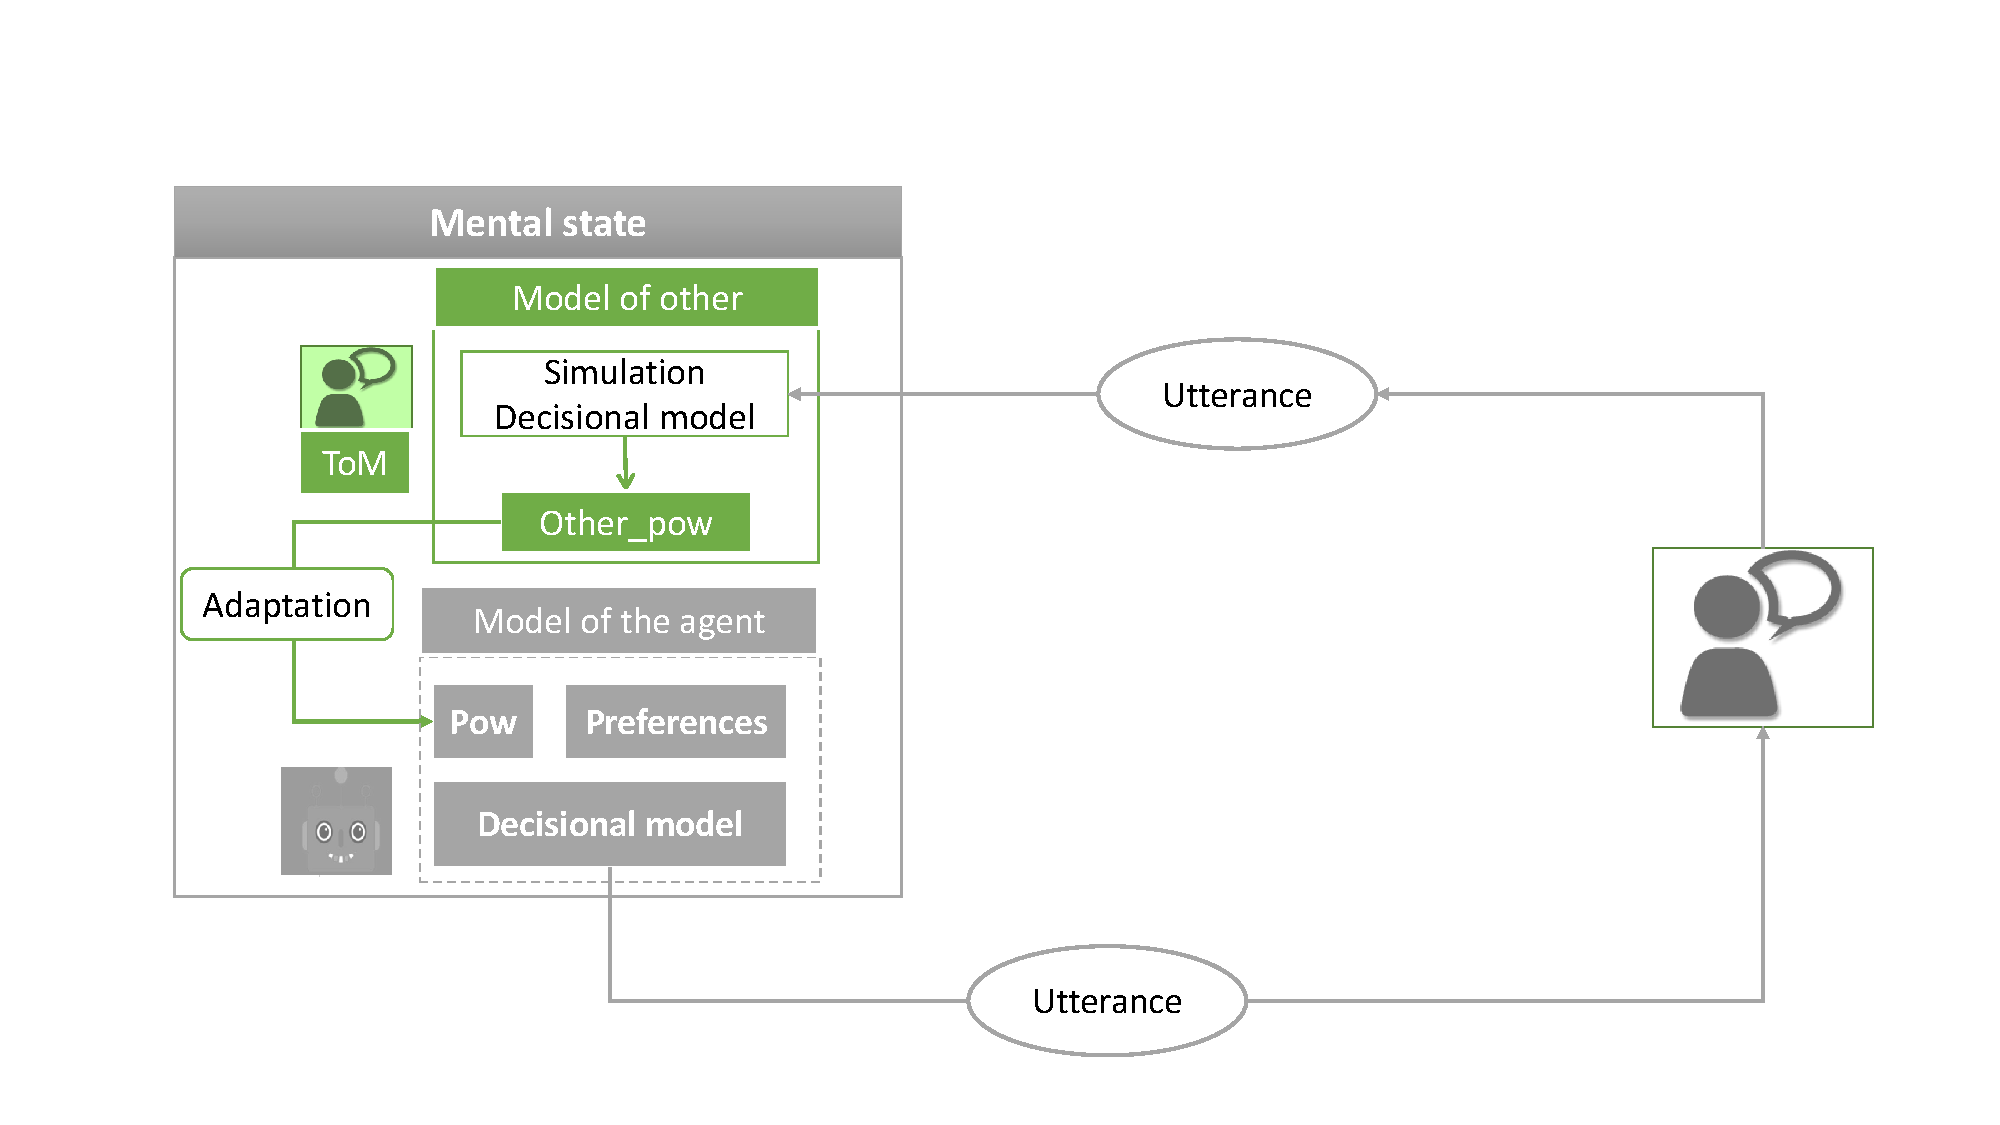
\includegraphics[width=\linewidth, height= 0.4\textheight]{figs/model_tom.pdf}}
			\caption{A theory of mind approach to evaluate the user's level of dominance} 
			\label{fig:tom}
	\end{figure*} 

	This approach however relies on a couple of strong assumptions. First, it assumes that the decision model is an accurate representation of the decisional process of the user. There is no way to guarantee this assumption. However, in our previous research \cite{ouali2017computational}, we showed that the dialogues produced by this model are correctly perceived by human users in terms of dominance. This is no proof that the model is similar to a human decision process, but the behaviors that it produces are at least coherent with the notion of dominance as human people understand it.
	
	The second assumption is that the system can build a model of the possible mental states of the interlocutor. Concretely, this means a value of $pow$ and a set of preferences $\prec_i$ for all criteria. The general algorithm for a ToM is as follows:
	\begin{enumerate}
	\item Build a set $H_{pow}$ of hypothesis about power: $h\in H_{pow}$ represents the hypothesis $pow=h$;
	\item For each hypothesis $h$, build the set of all possible preferences $Prec_h$: the elements $p\in Prec_h$ are partial orders on the criteria.
	\item After each user utterance $u$, remove all elements in $Prec_h$ that are not compatible with $u$. Concretely, if the applicability condition of $u$ is not satisfied in $p\in Prec_h$, then $p$ must be removed from the candidate mental states.
	\item For each $h$, compute a score $score(h)$ based on the size of remaining hypothesis $|Prec_h|$
	\end{enumerate}
	The idea is that the hypothesis with the highest score is the most probable value for the user's power value.

	\begin{equation}
	pow_{other} = \operatorname*{arg\,max}_{h} (score(h))
	\end{equation}

	There is, of course, an infinite set of possible values for $pow$. In our work, we consider only 9 values: $H_{pow} = \{0.1, 0.2, \ldots, 0.9\}$.

	\subsection{Complete model of preferences}
	
	To build the set of possible preferences for each hypothesis, we need to consider all possible partial orders $\prec_i$ for each criterion $C_i$. However, there are $(|C_i| + 1)!$ possible partial orders for each criteria. As a consequence:
	
	$$ |M_H| = \prod_{i=1}^n (|C_i|+1)!$$
	
	In the negotiation dialogue we consider for our work, there are approximately 5 criteria with 4 to 10 possible values each. This means that there are between $24.10^9$ and $100.10^{36}$ possible preference sets. It is not reasonable to consider them all, one by one, at each step of the dialogue.
	
	Even if we consider only total order sets of preferences, we still have  $\prod_{i=1}^n |C_i|!$ possible sets. It remains impossible to consider in the context of a dialogue.
	
	Moreover, our goal is not to model the exact mental state of the interlocutor. We only want to evaluate his/her behavior of power. In the proposed ToM approach, we need to make hypothesis on the preferences to compute the applicability conditions of the utterances. The system uses the preferences to evaluate which values are satisfiable ($S$) or acceptable ($Ac$), depending on the value of $pow$ and the current progress of the negotiation. But the preference set $Pref_h$ contains too much information! What is really required to simulate the decision process are only the sets $S$ and $Ac$, as shown on table~\ref{tab:utt}.
	
	Thus, we want to build hypotheses on $S$ and $Ac$, not on $Pref$. This does not reduce the complexity since we have as many possible $S$ and $Ac$ as preference sets, at a given time of the negotiation.
	
	Our proposal to reduce this complexity is to consider only $S$ in the hypothesis of preferences, and to assume that we have a total order on the preferences.
	
	Indeed, when all values are comparable, it is possible to sort them by order of preferences. In this case, the value of satisfiability only depends on the rank in this order of preferences, not on the order of the other elements in the set. For example, consider a criterion with 4 values and a total order of preferences on thees values. The value of can be sorted by order of preferences. The score of satisfiability for each rank is presented on Table~\ref{tab:poss}: it does not depend on the values themselves. For instance, the third value of the preference set will have $sat(v)=.66$, as defined in section~\ref{sec:dialogue-model}.
		\begin{table}[h]
			\caption{Satisfiability depending on the rank for a 4-values criterion.}
			\label{tab:poss}
			\centering
			\begin{tabular}{ |c|c|c|c|c| }
				\hline				
				rank(value) & 1 & 2 & 3 & 4 \\
				\hline
				Nb predecessors & 3 & 2 & 1& 0 \\
				\hline
				Sat(value) & 0 & 0.33 & 0.66 &1 \\
				\hline
			\end{tabular}
		\end{table}
	
	As a consequence, for a given value of power $pow$, the size of $S$ is fixed, independently of the possible relation of preferences $\prec$.
	This modeling will allows the agent will compute a smaller set oh hypotheses. However, simulating the behavior of other with incomplete knowledge will affect the precision of the prediction.  
%	XXX il reste une phrase pour dire qu'on a moins d'hypothèse mais qu'on le paye en ayant un modèle de décision qui doit être modifié pour la ToM XXX
	
	\subsection{Partial model of preferences}
	
	The model of preferences is used to compute the satisfiability of values (see section \ref{sec:sat}). Knowing the set of satisfiable values is crucial for the decisional process. Therefore, instead of computing hypotheses on the set of preferences, we propose to compute hypotheses about $S$, the set of satisfiable values for a giving value of power $pow$.  
	
	\par In order to generate theses hypotheses for any criterion, we make the strong assumption that preferences are \emph{total ordered.} In this case, all the values are comparable and could be ranked by order of preferences. Knowing the rank of preferences allows the agent to compute in advance the possible values of satisfiability.
	

	Based on the values of satisfiability, and given a fixed value of $h_i \in H_{pow}$, we can compute the size of $S$ in order to generate hypotheses on the different combination of satisfiable values  noted $M_h(h_i)$. For example, considering a value of $pow =0.6$, and the same criterion $M$, the number of satisfiable values $|S| = 2$. Therefore, $M_h(pow) = \{(A,B), (A,C), (A,D), (B,C), (B,D), (C,D)\}$. This process is generalized to all the hypotheses of $H_{pow}$. An example is presented in the table \ref{tab:sat}
	
	
	
	
	\begin{table}[h]
		\centering
		\caption{Hypotheses on mental states for the criterion $M=\{A, B, C, D\}$}
		\begin{tabular}{ |c|c|c| }
			\hline
			& \multicolumn{2}{c|}{Hypotheses}  \\
			\hline
			Hypothesis & pow & $M_h(pow)$ \\
			\hline
			H1&0.3&$\{ (A,B,C) , (A,B,D), (A,C,D), (B,C,D) \}$ \\
			\hline
			H2&0.4&$\{ (A,B), (A,C), (A,D), (B,C), (B,D), (C,D) \}$ \\
			\hline
			H3&0.5&$\{ (A,B), (A,C), (A,D), (B,C), (B,D), (C,D) \}$\\
			\hline
			H4&0.6&$\{ (A,B), (A,C), (A,D), (B,C), (B,D), (C,D) \}$ \\
			\hline
			H5&0.7&$\{ (A), (B), (C), (D) \}$\\
			\hline
			H6&0.8&$\{ (A), (B), (C), (D) \}$ \\
			\hline
			H7&0.9&$\{ (A), (B), (C), (D) \}$ \\
			\hline
		\end{tabular}

		\label{table:poss}
	\end{table}
	
	\subsection{Decision in negotiation with partial representation of preferences}
	The adaptation of the mental state to partial representation implies to modify the reasoning process. In the following, we present the adaptation of the decisional model to take into account partial and incomplete mental state. The goal is to reproduce the reasoning model in order to compute at each turn, the power $other_{pow}$ of the interlocutor. 
	
	First, we present the adaptation of the functionalities. Second, we present, the computation of the other's \emph{pow} from functions of decision.   
	
	\subsubsection{Satisfiability:}
	To compute whether a value $v \in C_i$ is satisfiable, we check for each hypothesis of power $h_i$, the set satisfiable values $S_i \in M_h(pow)$.
	Thus: 
	\begin{equation}
	sat_{S_i}(v)= \left\{\begin{array}{ll}
	True	 & \mathrm{if\ }  v \in S_i\\
	False & \mathrm{otherwise}
	\end{array}\right.
	\end{equation}
	
	\subsubsection{Acceptability:}
	Computing the acceptability of a value $v$ depends on the current of value of $self(t)$. For each hypothesis on power $h_i$, we associate a value $self_i(t)$ that represents the level of concessions at the current time. 
	
	With partial knowledge of preferences and for a fixed value of power $h_i$, the agent is not able to compute all the acceptable values $Ac_i$. Especially,   values of the set $M_i$ (\emph{i.e} acceptable values which are not satisfiable). 
	
	Nevertheless, the agent can have certain information about acceptable values such as $ S_i \subset Ac_i$. Moreover, using the initial values of satisfiability for a given criterion (see table \ref{sat}), agent can compute the number of acceptable values at the current state of the negotiation $|Acc_i|$ and by consequences $|M| = |Acc_i| - |S_i|$. 
	
	We propose to calculate the score of acceptability of a value $v$ taking into account the available information. Therefore, for a hypothesis of power $h_i$, hypotheses on preferences $S_i \in M_h(h_i)$,  and the list of accepted values during the negotiation $A$, the score that $v \in D$ is acceptable is computed as follow: 
	\begin{equation}
	Acc(v, pow) = C_{|D|-(|S_i| + k)}^{|M| - k}
	\end{equation}
	$k = |K| $ is the number of elements in the set $K = A \cap \overline S_i$
	
	
	
	\subsection{Update hypotheses about pow}
	At each turn of the dialogue, the agent uses its model of the theory of mind in order to compute other's behaviors of power $pow_{other}$. We present, the process of updating $other_{pow}$ depending on the received utterance. 
	\subsection{Lead of the dialogue}		
	As presented before, the choice of a specific utterance's type translates behaviors of power. Indeed, a high frequency of choosing \emph{proposal utterance} shows a behaviors of high-power. Whereas, a high frequency of \emph{share preferences utterances} reflects behaviors of low-power.
	We note $history$ the list of utterances enunciated by the user. the value of power is computed from the ratio of propose enunciated versus asks.
	\begin{equation}
	pow_{other} = \left\{\begin{array}{ll}
	> 0.5 & \mathrm{if } \frac{history(Propose)}{hisotry} > 0.5\\
	\leq 0.5 & \mathrm{if  } \frac{history(Ask)}{hisotry} > 0.5
	\end{array}\right.
	\end{equation}
	
	Once, the list of possible is restricted, we update the hypotheses by taking into account the value associated to the expressed utterance.
	
	\subsubsection{Share a preference}
	When the user expresses a \emph{StatePreference(v, s)}, he shares his preferences in the way where $v \in S$ if $s =true$, otherwise $v \notin S$. 
	In addition, when the user rejects a proposal \emph{Reject(p)}, he also shares his preferences . As $S \subset Acc$ means if a value is not acceptable, it is automatically not satisfiable $p \notin S$. 
	
	Therefore, for each  $h_i \in H_{pow}$, we propose to update the agent's hypotheses $M_h(h_i)$ by removing all the hypotheses on preferences that are no longer consistent with the information learned. 
	Then, we compute the score of each $h_i$ at the moment $t$ :
	
	$$score(h_i,t) = \frac{|M_h(h_i, t)|}{|M_h(h_i, init)|}$$
	
	The value of power selected:
	\begin{equation}
	pow_{other} = \operatorname*{arg\,max}_{h_i \in H_{pow}} ( score(h_i,t))
	\end{equation}
	
	\subsection{Accept a proposal}
	When the user accept (\emph{Accept(p)}) or propose a proposal (\emph{Propose(p)}), means that $p \in Acc$. 
	The agent has to calculate for each $h_i \in H_{pow}$ the score of acceptability. In addition, the values of acceptability have to be normalized to allow a coherent comparison. Thus, given a hypothesis on power $h_i$, he score of acceptability is normalized by taking into account the ideal score of acceptability.
	
	$$I_{pow} =  C_{|D|-|S_i|}^{|M|}$$
	
	
	The final value of acceptability is then:
	\begin{equation}
	score(h_i, t)= \left( \begin{array}{c}  \frac{1}{I_{pow}} \cdot \sum_{S_i \in M_h(h_i) } acc(p, h_i) 
	\end{array}\right) \frac{1}{| M_h(h_i)|}
	\end{equation}
	
	Finally, the value of power is selected using the function (7) presented earlier.
	
	
	\section{Evaluation}
	In this section, we present our simulation study to show the acceptability of our model of dialogue. We aim to evaluate the accuracy of our model of theory of mind as well as the timeliness of the algorithm.
	
	\subsection{Method}
	
	We implemented two agents with theory of mind abilities.
	The first agent ($agent_A$) plays a role of a dominant agent( $pow > 0.5$), whereas, the second agent ($agent_B$) plays the role of a submissive agent ($pow \leq 0.5$). 
	We manipulated two simulation parameters for the initialization of our agents. First, the power of both agents (named \emph{pow-a} and \emph{pow-b}). We variate the values of power in order to study the accuracy of predictions in different settings as presented in table \ref{tab:powsettings}.
		\begin{table}[t]
			\centering
			\caption{Initial condition's setting for the values of power} 
			\begin{tabular}{|l|cccc|}
				\hline 
				\textbf{Dominance value } &	\multicolumn{4}{c|}{ Initial values of power } \\
				\hline
				Dominant agent $pow_A$ & 0.3 & 0.4 & 0.5 &  \\
				\hline
				Submissive agent $pow_B$ & 0.6 & 0.7 & 0.8 & 0.9\\
				\hline
			\end{tabular}
			
			\label{tab:powsettings}
		\end{table}
		
	Second, we variate the size of preference sets and more specifically the size of the discussed topic in order to study the timeliness of the algorithm from simple to richer topics. We generate three types of topics as presented in table \ref{tab:initP} and for each topic we generated $50$ different models of preferences. In total, negotiators was initiated with $150$ different models of preferences, added to the values of power,  $1451$ combinations were created for the initial states of both agents. For each combination, we generate a dialogue in which the agent with theory of mind estimates the other's value of power.

	
		\begin{table}[]
			\caption{Initial condition's setting for the preferences set} 
			\centering
			\begin{tabular}{|p{1.75cm}|p{1.5cm}|p{1.75cm}|p{1.5cm}|}
				\hline 
				\textbf{Preference's name } & Number of criteria & Average number of values/criterion & Possible $M_h$\\
				\hline
					Small & 4 & 3 & 1296 \\
				\hline
					Medium & 4 & 4 & 4.14 E$^5$ \\
				\hline
				large & 4 & 10 & 2.6 E$^9$ \\
				\hline
			\end{tabular}

			\label{tab:initP}
		\end{table}
		
	\subsection{Results and discussion}
	We present in this section the results obtained for both the accuracy of predictions made by our model and the timeliness of the execution.
	
	\subsubsection{Accuracy of predictions:} For each dialogue, we obtain the predictions made by the agent with ToM abilities about the behaviors of power of the other agent. Results are summarized in table \ref{tab:res1}. 
	
	
	First, we computed the \emph{standard deviation} between the guessed value of power $Other_{pow}$ and the actual value of power $pow$. In average, for the total of $1451$ dialogues, a small deviation of $0.075$ was observed. Moreover, in order to analyze the results in a more general way, we calculated the \emph{residual deviation }  that computes the accuracy of the dependent variable being measured. We have computed the deviation of prediction between the predicted value  $Other_{pow}$ from the real value of power $pow$. 
	We observe deviations of the range $rv = 0.015$ which means that our model makes accurate and close predictions of other's power.
	
	
	\begin{table}[h]
		\centering
		\caption{Results of margin errors for prediction} 
		\begin{tabular}{|l|c|}
			\hline
			Average of the standard deviation & 0,075 \\
			\hline
			Residual variation (rv) & 0,015 \\
			\hline
		\end{tabular}

		\label{tab:res1}
	\end{table}
	
	Second, we analyzed the frequency of false predictions. For example, $agent_A$ predicts that $agent_B$ is dominant whereas $agent_B$ is submissive. To this end, we computed the percentage of false predictions. For all the dialogues, only $30$ predictions were incorrect which means that $ 2.6 \% $ of predictions were false. This result confirm the reliability of our algorithm. 
	\begin{table*}[t]
		\begin{tabular}{|c|c|c|}
			\hline
			\multicolumn{3}{|c|}{Number of etiration to make predictions} \\
			\hline
			Good predictions & $rv \leq 0.02$ & Best prediction \\
			\hline
			2.53 & 3.25 & 3.79\\
			\hline
		\end{tabular}
		\caption{Average number of iterations to compute a prediction} 
		\label{tab:conv}
	\end{table*}
	Finally, for all the dialogues in which the agent was able to find a good prediction (in total $1421$), we analyzed the rapidity of convergence of our algorithm. The results are presented in table \ref{tab:conv}

	 
	For each dialogue, we computed the number of iteration necessary to find a good prediction. In average, the algorithm needed $3$ iterations in order to predict the right range of dominance of the other (weather the agent has dominant or a submissive behavior). 
	
	Moreover, we calculated the average number of iterations needed to find a prediction such that $rv \leq 0.02$. In average the agent needed $3$ iterations in order to evaluate a close value to the other's power. The evolution of convergence for all the dialogues are presented in figure  \ref{fig:converge}
	
	We  also computed the average number of iterations in order to find the best prediction of $Other_{pow}$. The results depicted in table \ref{tab:conv} show that the agent makes in average $4$ iterations to converge towards the best value.  

%		\begin{table*}[t]
%		\begin{tabular}{|c|c|c|c|c|c|c|c|c|c|}
%			\hline
%			\textbf{$Other_{pow}$} & \multicolumn{9}{c|}{Number of iteration } \\
%			\hline
%			Small &0,047&0,071&0,063&0,016&0,010&0,009&0,011&0,011&0,011 \\
%			\hline
%			Medium&0,058&0,084&0,075&0,030&0,017&0,016&0,017&0,017&0,017\\
%			\hline
%			Large&0,052&0,116&0,099&0,024&0,015&0,015&0,017&0,017&0,018 \\
%			\hline
%			
%		\end{tabular}
%		\caption{Results of margin errors for prediction} 
%		\label{tab:conv}
%	\end{table*}
	
	We studied the impact of the initial number of hypotheses about the other model on the convergence of the algorithm. We wanted to study weather a large number of hypotheses will need extra iterations to converge. Therefore, we compared results obtained for small topic, medium, and large topics of negotiation. The graph presented in figure \ref{fig:converge} shows that our algorithm converges in average quickly independently from the size of topic. We can observe that the algorithm took two additional iterations to converge in the large topic. The difference is not significant to affect the general behavior of our model.
%	\begin{table}
%		\
%		\begin{tabular}{|p{3 cm}|c|c|c|}
%			\hline
%			Model size & Small & Medium & Large \\
%			\hline
%			Time execution (milliseconds) & 50.28 &	59.83 &	116.38\\
%			\hline
%		\end{tabular}
%	\end{table}
	
		\begin{figure}[]
			\fbox{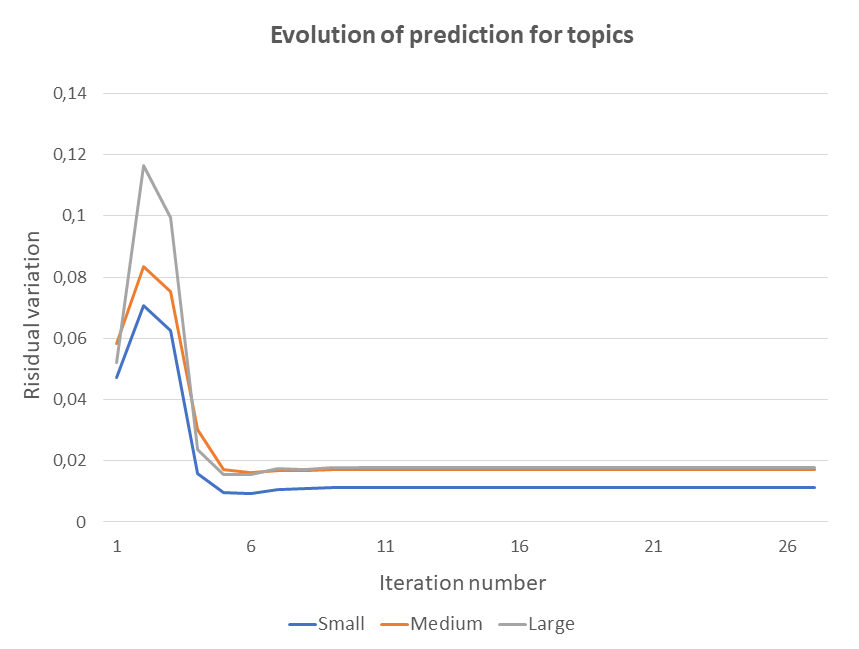
\includegraphics[width=\linewidth]{figs/total}}
			\caption{Algorithm convergence for all topics} 
			\label{fig:converge}
		\end{figure}
	
	
	\subsection{Timeliness}
	We evaluate the time execution of the algorithm in order to study how the model of theory of mind evolves.For each dialogue, we computed the the average time execution at each negotiation turn. We aim to study the effect of hypotheses's size on the rapidity of prediction at eahc turn. Results are presented in figure \ref{fig:time}. When comparing the time execution between the medium and large models, we observe that the algorithm took in average $12$ milliseconds at each turn. However, this difference is not significant since the total execution remains very quick.
	
	\begin{figure}[]
		\fbox{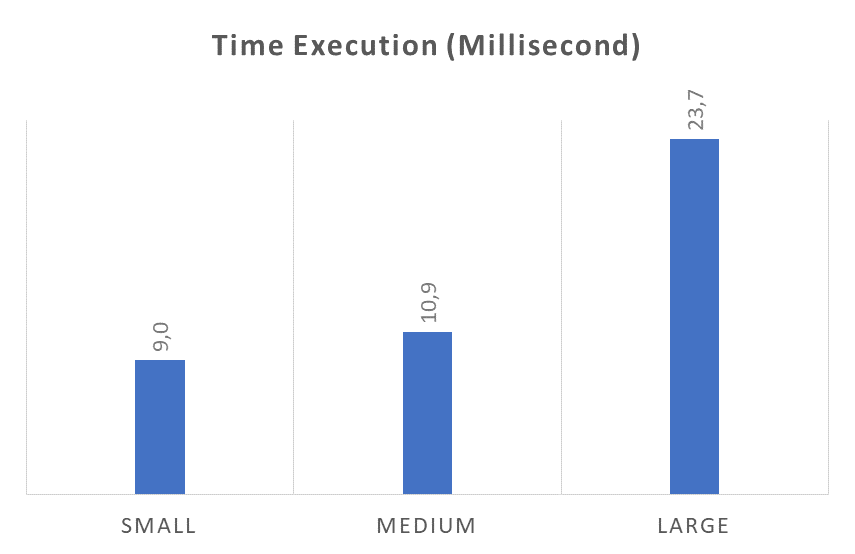
\includegraphics[width=\linewidth]{figs/time_exec.png}}
		\caption{Algorithm convergence for all topics} 
		\label{fig:time}
	\end{figure}

	We analyzed the behaviors of our model of ToM in different aspects and the obtained results provide a strong support to its accuracy. Indeed, for most of the generated dialogues, the agent with ToM abilities was able to evaluate a very close approximation of its partner's level of power. Moreover, the agent was able to find the right dominance range only after two dialogue turns and the best evaluation after five turns. Theses behaviors were generated in a reasonable amount of time allowing the agent to produce real time dialogues.
	
	 These findings strengthen the accuracy of our model and give good perspectives to implement this model in the context of human/ agent collaborative negotiation. However, the presented validation in the context of agent/agent negotiation is a controlled evaluation since both agents use the same decisional model. This situation increases the chance of good predictions of the partner's behaviors of power. 	Thus, a validation of our collaborative model of negotiation must be validated in the context of human/agent negotiation.
	\section{Conclusion}
		We presented in this paper, a model of collaborative negotiation with theory of mind (ToM) abilities. Our model of ToM focuses essentially to predict the agent's partner value of power in the perspective of defining a complementary relation of dominance.

		The agent builds partial representation of the mental state of its partner, allowing the agent to have sufficient knowledge to compute the value of the partner's power. In addition, the limited knowledge ensure the agent to reason in a reasonable time to produce real time dialogues.
		
		Our model was evaluated and validated in the context of agent/agent negotiation. The results confirmed the accuracy of the ToM models. Indeed, the agent was able to generate close and quick predictions of it's partner behaviors in several conditions.
		
		The presented evaluation relies on the fact that both agents use the same decision to build their strategy in  the negotiation. However, in the context oh human/agent negotiation, the agent doesn't know the decisional model of the user. We only make the assumption that the user uses the same reasoning as the agent.
		%Rappeler l'importance de la complementarite
		 Therefore as perspective, we aim to evaluate the accuracy of our model in the human/user negotiations. Moreover, the agent will also adapt its behaviors of power to complement the predicted user's behaviors in order to simulate the dominance complementarity. In such situation, the agent will have to consider the effect of wrong predictions on the negotiation outcomes. We believe that modeling a complementary relation of dominance will improve the negotiation outcomes and increase mutual liking between the agent and the user.
		
		
	%%%%%%%%%%%%%%%%%%%%%%%%%%%%%%%%%%%%%%%%%%%%%%%%%%%%%%%%%%%%%%%%%%%%%%%%%%%%%%%%%%%%%%%%%%%%%%%%%%%%%%%%%
	%% bibliography: see CFP for number of permitted pages
	
	\bibliographystyle{ACM-Reference-Format}  % do not change this line!
	\bibliography{bibliography}  % put name of your .bib file here
	
\end{document}